\section{Ensemble}
\label{sec:ensemble}
Our approach builds upon an ensemble voting strategy of different runs of multiple Recurrent Neural Networks (RNNs) and one execution of Title2Rec. The RNNs are configured differently in terms of network inputs and hyper-parameters. The RNNs are used to predict the missing tracks to be part of a playlist and thus assume to have seed(s) track(s) of the playlist to be utilized as initial elements of the network bootstrap (Section~\ref{sec:rnn}). However, when only the title of the playlist is available, our approach relies on a fall-back strategy that implements a K-means clustering of the playlists and a word embedding model of their titles (trained with fastText), called Title2Rec (Section~\ref{sec:t2r}). Figure~\ref{fig:ensemble} illustrates the overall approach.

\begin{figure}
    \centering
    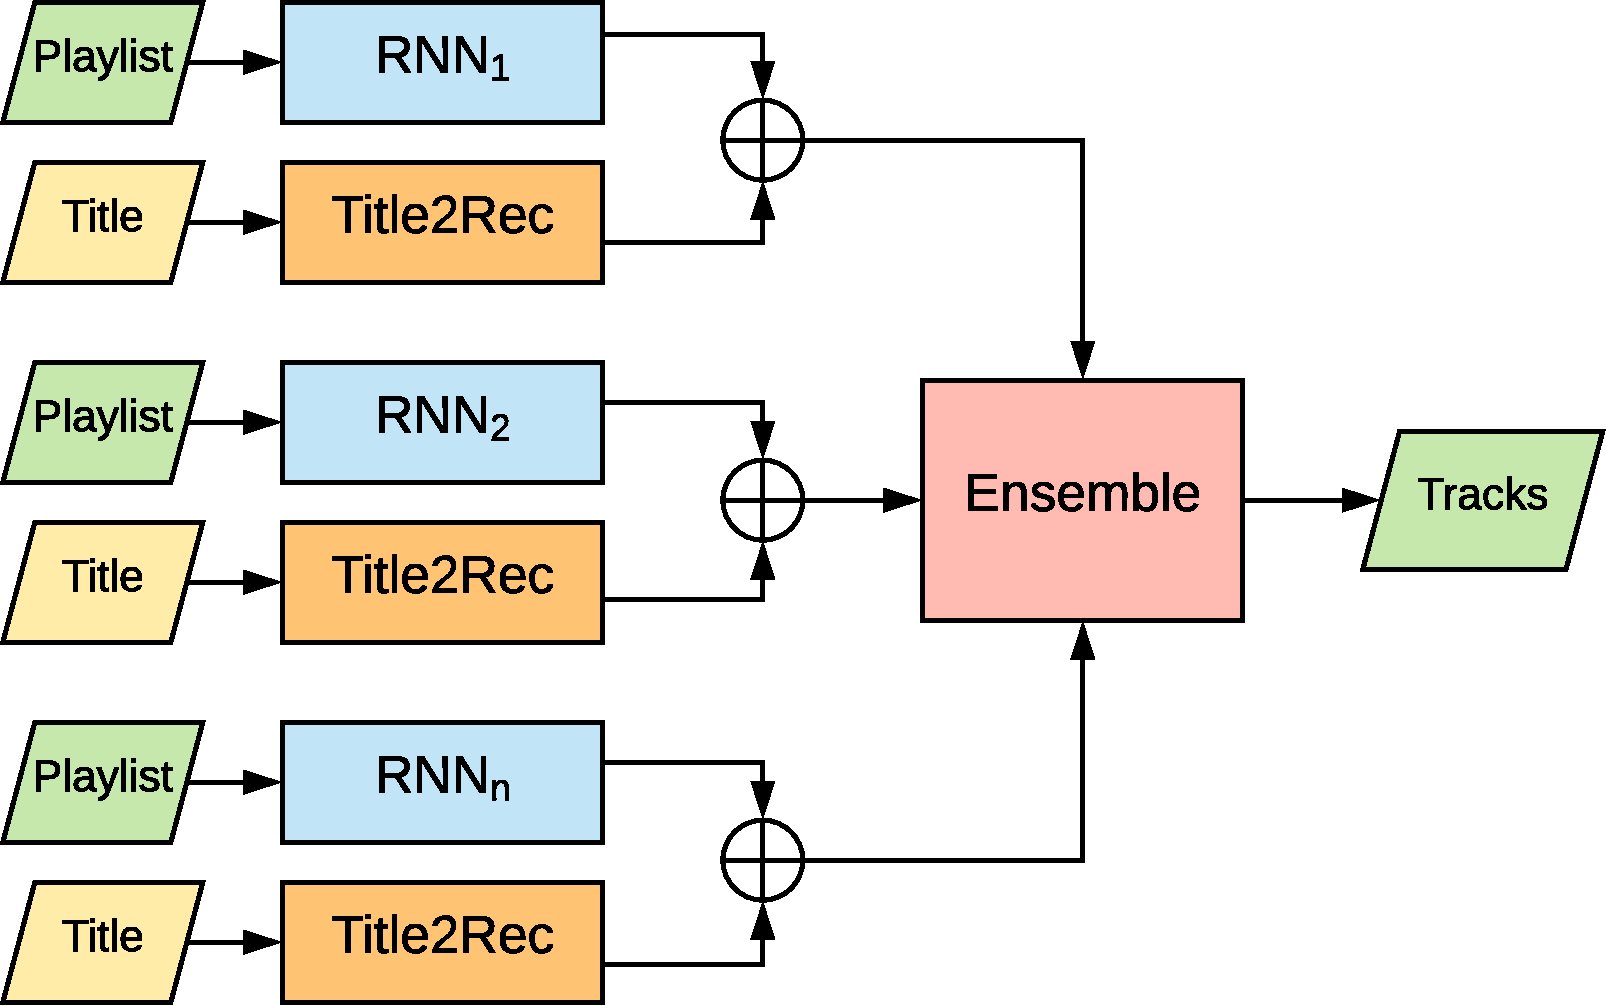
\includegraphics[width=\textwidth, width=0.47\textwidth]{figures/ensemble.pdf}
    \caption{The proposed ensemble architecture for playlist completion. The inputs are a playlist and its title.}
    \label{fig:ensemble}
\end{figure}

The ensemble weighs the rankings of the different runs by giving more importance (more weights) to the top ranked tracks and less to the low ranked tracks, similarly to a Borda count election.\footnote{\url{https://en.wikipedia.org/wiki/Borda_count}} In detail, given a ranked set of predictions coming from a configuration $k$, corresponding to a particular configuration of the RNN jointly combined with Title2Rec, $R_k = \{T_1, T_2, \dots, T_{500}\}$, we assign to each track a score $s_k$ that has its maximum for the first track in the ranking and minimum for the last one, i.e. $s_k(T_i) = 500 - i + 1$. Then, we sum the scores over all the configurations that we want to ensemble, obtaining a final score for each track $s(T_i) = \sum_{k} s_k(T_i)$ which we use to create the final ranking of the tracks. Take as an example (with 3 tracks instead of 500 in the predictions) a configuration $1$ with ranking $R_1 = \{T_1, T_2, T_3\}$ and a configuration $2$ with ranking $R_2 = \{T_1, T_3, T_2\}$. We would get $s_1(T_1) =  3$, $s_1(T_2) = 2$, $s_1(T_3) = 1$, $s_2(T_1)=3$, $s_2(T_3) = 2$, $s_2(T_2)=1$ and thus $s(T_1) = 3+3= 6$, $s(T_2)= 2+1=3$, $s(T_3)=1+2=3$, obtaining as a final ranking $R = \{T_1, T_2, T_3\}$, or equivalently $R = \{T_1, T_3, T_2\}$ as $T_2$ and $T_3$ have the same score.